\chapter{Graphs}
\label{chap-graphs}
In some ways, Graphs are the most important data structure.  
Graphs represent and model relationships, and humans are defined by relationships.
The archetypical examples of graphs used to be maps and the distances between landmarks or looking for the shortest path.

With the advent of social media, we can talk about graphs with a few examples that might be easier to intuit.

\section{Introduction and History}


\section{Qualities of a Graph}

The physical layout of a graph doesn't actually matter\footnote{Some properies, such as whether a graph is \emph{planar} or \emph{bipartite} effectively care if a graph can be physically laid out in a certain way.}

\subsection{Vertices}

\begin{itemize}
	\item Vertices must be unique.
\end{itemize}

\subsection{Edges}

\subsubsection{Undirected Edges}

\subsubsection{Directed Edges}

\subsubsection{Weighted Edges}


\section{Special Graphs and Graph Properties}

\subsection{Planar Graphs}
Graphs that are planar can have their vertices and edges laid out in such a way that no two edges will cross.



\subsection{Bipartite Graphs}

\subsection{Directed Acyclic Graphs}

%TODO our dragon slaying example

\section{Building a Graph}

\subsection{Adjacency List}
\subsection{Adjacency Matrix}
\subsubsection{Matrix multiplication and GPU Abuse}

\section{Graph Libraries}

\subsection{Java - JUNG}

\subsection{Python - networkx}

There is only one realistic choiceforusing graphs in Python.  The package networkx is extremely powerful, extremely versatile,and actively maintained.




\section{Graphs, Humans, and Networks}

\subsection{The Small World}
\subsubsection{The Milgram Experiment}
%In 1960, the fugative Nazi war criminal Adolf Eichmann was captured by 
\subsubsection{The Less-Known Milgram Experiment}

\subsection{Scale Free Graphs}


\section{Graphs in Art and Nature - Voronoi Tessellation}

\begin{figure}
	\centering
	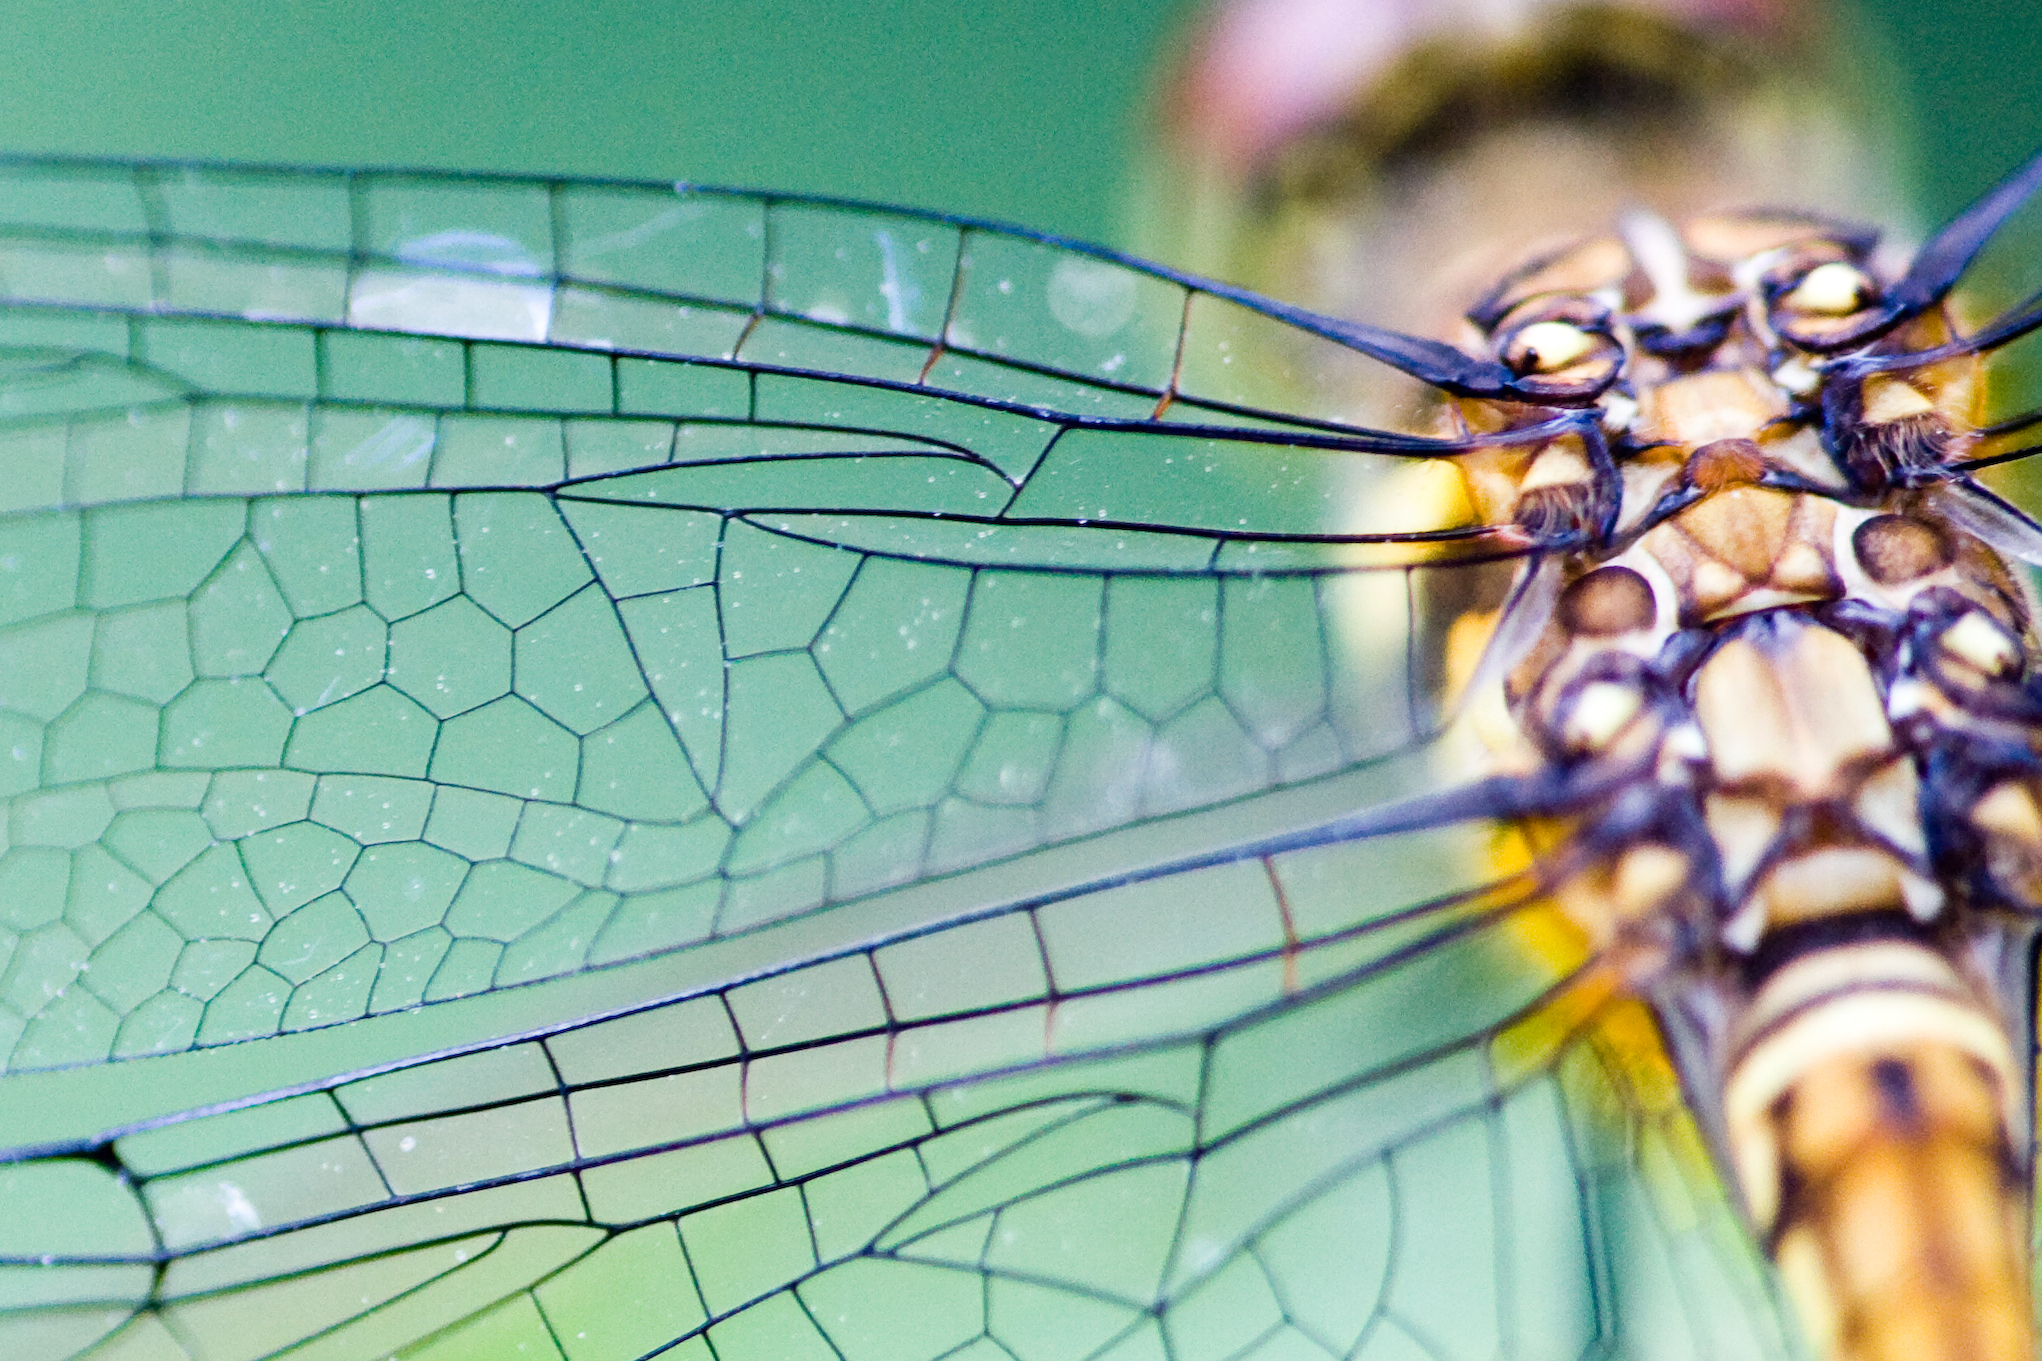
\includegraphics[width=0.7\linewidth]{pics/dragonfly_wing_joi_ito}
	\caption{The wings of a dragonfly. Credit: Joi Ito (CC BY 2.0)}
	\label{fig:dragonflywingjoiito}
\end{figure}


